\documentclass[9pt, aspectratio=169]{beamer}
%\documentclass[9pt, aspectratio=169, handout]{beamer}

\usetheme{metropolis}
\setbeamertemplate{itemize items}{\faAngleRight}

\metroset{titleformat=smallcaps,block=fill,numbering=counter,progressbar=frametitle,sectionpage=none}
\setbeamersize{text margin left=5mm,text margin right=5mm} 
% \input{embed_video}
\usepackage{fontspec,minted}
\usepackage[scale=1]{ccicons}
\usepackage{metalogo}
\usepackage{xcolor,colortbl}
\usepackage{multicol,multirow,booktabs}
\usepackage{appendixnumberbeamer}
\usepackage{graphicx}
\usepackage{mismath}
\usepackage{bm}
\usepackage{fontawesome5}
\usepackage{csquotes}
%\usepackage[backend=biber, natbib, sorting=nyt, doi=true, url=false, url=false, isbn=false, maxbibnames=10]{biblatex}
%\addbibresource{../../utils/refs.bib}

\usepackage[spanish, es-nodecimaldot]{babel}
\deftranslation[to=spanish]{Definition}{Definición}
\deftranslation[to=spanish]{Theorem}{Teorema}
\deftranslation[to=spanish]{Example}{Ejemplo}

\usepackage{mathtools, mathrsfs}
\usefonttheme{professionalfonts}
\usepackage{textcomp, wasysym}

\setsansfont[BoldFont={Iwona Bold}, Numbers={Lining, Proportional}]{Iwona Light}
% \setmathsfont(Digits)[Numbers={Lining, Proportional}]{Fira Sans Light}
\setmonofont[Scale=MatchLowercase]{DejaVu Sans Mono}

\setbeamercolor{alerted text}{fg=red,bg=black!2}
\setbeamercolor{progress bar}{fg=red,bg=red!2}
\setbeamertemplate{itemize item}{\faCaretRight}
\setbeamertemplate{itemize subitem}{ \faAngleRight}
\setbeamertemplate{blocks}[shadow=false]
\setbeamercolor{block title}{bg=black!30,fg=red}
\setbeamercolor{block body}{bg=black!20,fg=black}
\setbeamertemplate{theorem begin}
{%
\begin{\inserttheoremblockenv}
{%
\inserttheoremheadfont
%{Teorema:}
\inserttheoremname
\ifx\inserttheoremaddition\@empty\else\ : \inserttheoremaddition\fi%
\inserttheorempunctuation
}%
}
\setbeamertemplate{theorem end}{\end{\inserttheoremblockenv}}
\makeatother


 
\usepackage{gensymb,amssymb}
\usepackage{upquote}
\usepackage{cancel}
\usepackage{algpseudocode}
\algrenewcommand\algorithmicrequire{\textbf{Requiere}}
\algrenewcommand\algorithmicensure{\textbf{Devuelve}}
\setbeamertemplate{blocks}[shadow=false]

\newcommand{\cx}{\column{0.5\textwidth}}
\newcommand{\cw}[1]{\column{#1\textwidth}}

\author{Manuel Carlevaro}
\date{}
\institute{
  \vspace{6em}
  \centering
  {\tiny
  Universidad de Navarra \enspace • \enspace 2024 
} }

%% Operadores
\DeclareMathOperator{\sen}{sen}
\DeclareMathOperator{\senc}{senc}
\DeclareMathOperator{\sign}{sign}
\newcommand{\T}[1]{\underline{\bm{#1}}}
\DeclareMathOperator{\Tr}{Tr}
\DeclareMathOperator{\rg}{rg}
\DeclareMathOperator{\cond}{cond}

\usepackage{hyperref}
\hypersetup{
    colorlinks,
    citecolor=blue,
    filecolor=black,
    linkcolor=blue,
    urlcolor=blue
}
\urlstyle{same}


\usepackage{tikz}
\usetikzlibrary{shapes,shadows,arrows,positioning,matrix,chains,backgrounds,fit}

\tikzset{
    %Define standard arrow tip
    >=stealth',
    %Define style for boxes
    obj/.style={
           rectangle,
           rounded corners,
           draw, very thick,
           text width=10em, fill=green!20,
           minimum height=2em,
           text centered, drop shadow},
    proc/.style={
	    rectangle, rounded corners,
	    draw,fill=red!50,very thick,
	    text width=8em,minimum height=2em,
	    text centered, drop shadow},
    % Define arrow style
    pil/.style={
           ->,
           thick,
           shorten <=2pt,
           shorten >=2pt,}
}

%\setbeamertemplate{bibliography item}{%
  %\ifboolexpr{ test {\ifentrytype{book}} or test {\ifentrytype{mvbook}}
    %or test {\ifentrytype{collection}} or test {\ifentrytype{mvcollection}}
    %or test {\ifentrytype{reference}} or test {\ifentrytype{mvreference}} }
    %{\setbeamertemplate{bibliography item}{\faBook}}
    %{\ifentrytype{online}
            %{\setbeamertemplate{bibliography item}{\faGlobe}}
   %{\setbeamertemplate{bibliography item}{\faFileText}}}%
  %\usebeamertemplate{bibliography item}}

%\defbibenvironment{bibliography}
  %{\list{}
     %{\settowidth{\labelwidth}{\usebeamertemplate{bibliography item}}%
      %\setlength{\leftmargin}{\labelwidth}%
      %\setlength{\labelsep}{\biblabelsep}%
      %\addtolength{\leftmargin}{\labelsep}%
      %\setlength{\itemsep}{\bibitemsep}%
      %\setlength{\parsep}{\bibparsep}}}
  %{\endlist}
  %{\item}
%\newcommand{\bcite}[1]{\citeauthor{#1}, \citetitle{#1} (\citeyear{#1})}


\title{Introducción a la física}
\subtitle{Cinemática}


\begin{document}
\maketitle
\begin{frame}
  \frametitle{Objetivos}
\Large

\begin{itemize}
 \item Repasar los conceptos de desplazamiento, velocidad y aceleración.
 \item Reforzar la construcción e interpretación de gráficos de movimiento.
 \item Aprender a operar estas cantidades en forma vectorial.
\end{itemize}
\end{frame}

\begin{frame}{Desplazamiento y velocidad}
\begin{columns}
\cx
\begin{center}
    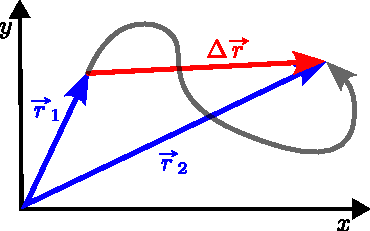
\includegraphics[width=0.8\textwidth]{figs/fig-01.pdf}
\end{center}
\cx
\textbf{Velocidad media:}
\begin{align*}
    \bm{v}_m &= \frac{\Delta \bm{r}}{\Delta t} \mapsto \text {velocidad media}\\
    v_m &= \frac{\norm{\Delta \bm{r}}}{\Delta t} \mapsto \text {rapidez media}
\end{align*}
\end{columns}
\pause

\begin{example}
    Adela viaja en bici \qty{2.0}{h}. Luego de muchas vueltas acaba a \qty{10.0}{km} al este de su origen. ¿Cuál fue su velocidad media? Al día siguiente consigue la misma rapidez media pero acaba \qty{3.0}{km} al norte y \qty{4.0}{km} al oeste. ¿Cuál fue su velocidad y el tiempo de viaje?   
    {\small
    \begin{columns}
        \cw{0.35}
        \begin{align*}
            \bm{v}_{m1} &= \frac{\Delta \bm{r}_1}{\Delta t_1} = \frac{(\num{10.0} \bm{i} + \num{0.0} \bm{j}) \unit{km}}{\qty{2.0}{h}} \\
                   &= (\num{5.0} \bm{i} + \num{0.0} \bm{j}) \unit{km/h} \\
            v_{m1} &= \qty{5.0}{km/h} 
        \end{align*}
        \cw{0.35}
        \begin{align*}
            \norm{\Delta \bm{r}_2} &= \sqrt{(\qty{3.0}{km})^2 + (\qty{4.0}{km})^2} = \qty{5.0}{km} \\
            \Delta t_2 &= \frac{\norm{\Delta \bm{r}_2}}{v_{m1}} = \frac{\qty{5.0}{km}}{\qty{5.0}{km/h}} = \qty{1.0}{h}
        \end{align*}
        \cw{0.3}
        \begin{align*}
            \bm{v}_{m2} &= (\num{3.0} \bm{i} - \num{4.0} \bm{j}) \unit{km/h}
        \end{align*}
    \end{columns}
    }
\end{example}
\end{frame}

\begin{frame}{Desplazamiento y velocidad: caso unidimensional}
\begin{columns}
\cx
\begin{center}
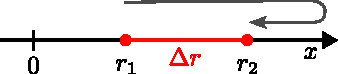
\includegraphics[width=0.9\textwidth]{figs/fig-02.pdf}
\end{center}
\begin{itemize}
\item Velocidad media: \[v_m = \frac{\Delta r}{\Delta t} = \frac{r_2 - r_1}{\Delta t} \]
\item Rapidez media: \[ |v_m| = \frac{|\Delta r|}{\Delta t} = \frac{|r_2 - r_1|}{\Delta t} \]
\end{itemize}
\pause
\cx
\begin{example}
{\small
Adela viaja en bici \qty{2.0}{h}. Luego de muchas vueltas acaba a \qty{10.0}{km} al este de su origen. ¿Cuál fue su velocidad media? Al día siguiente consigue la misma rapidez media pero acaba a \qty{5.0}{km} al oeste. ¿Cual fue su velocidad media y el tiempo de viaje?
\begin{center}
    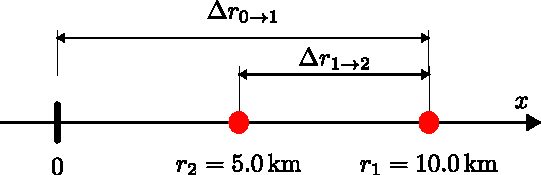
\includegraphics[width=0.7\textwidth]{figs/fig-03.pdf}
\end{center}
\begin{align*}
    v_m &= \frac{\qty{10.0}{km}}{\qty{2.0}{h}} = \qty{5.0}{km/h} \quad |v_m| = \qty{5.0}{km/h}\\
    \Delta t_2 &= \frac{|r_2 - r_1|}{|v_m|} = \frac{|\num{5.0} - \num{10.0}| \unit{km}}{\qty{5.0}{km/h}} = \qty{1.0}{h} \\
    v_{m2} &= \frac{(\num{5.0} - \num{10.0}) \unit{km}}{\qty{1.0}{h}} = -\qty{5}{km/h}
\end{align*}
}
\end{example}
\end{columns}
\end{frame}

\begin{frame}{Representación gráfica}
\begin{columns}
\cx
\begin{center}
    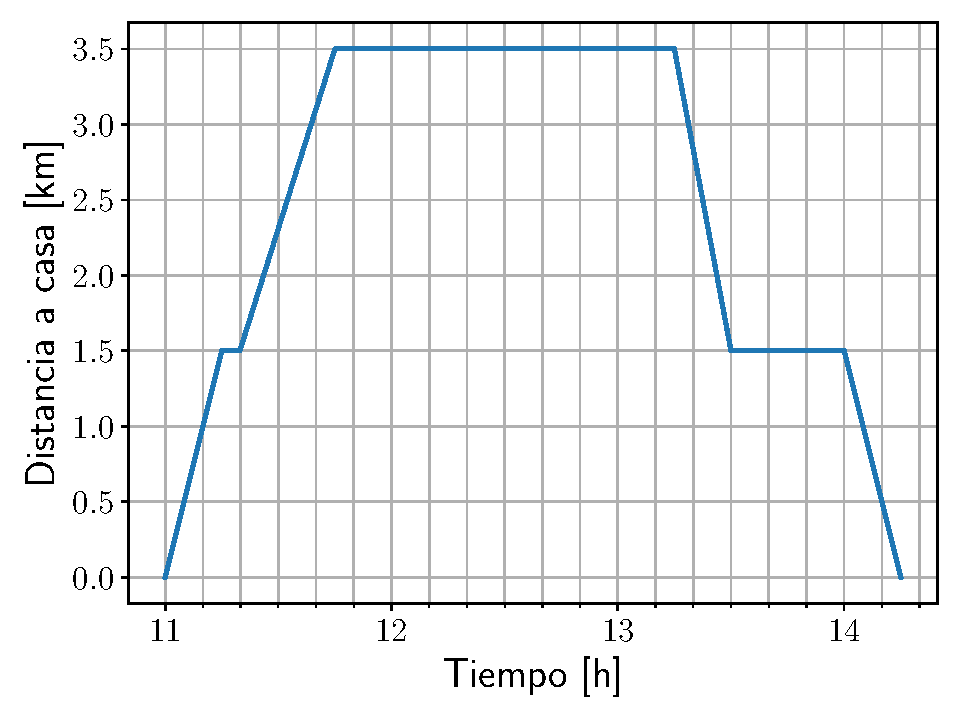
\includegraphics[width=0.5\textwidth]{figs/bruno.pdf}
\end{center}
\cx
{\small
    Los abuelos de Bruno lo invitaron a él y a sus primas a almorzar. La casa de Bruno, la de sus primas y la de sus abuelos quedan todas en la misma calle. Bruno sale caminando a las \qty{11}{h}, pasa a buscar a sus primas por su casa y se van a lo de sus abuelos. Al regreso, vuelven juntos. El gráfico representa la distancia de Bruno a su casa en cada momento.
}
\end{columns}
\begin{multicols}{2}
{ \small
\begin{itemize}
 \item ¿Cuándo estuvo a 1 km de su casa? ¿Y a 3 km de su casa?
 \item ¿A qué distancia de su casa se encontraba a la media hora de haber salido? ¿Y a las 11:50? ¿Y a las 13:10 y 13:20? ¿A qué hora volvió Bruno a su casa?
 \item ¿A qué distancia de la casa de Bruno está la casa de sus primas? ¿Y a qué distancia queda la casa de sus abuelos de la casa de sus primas?
 \item ¿Durante cuánto tiempo estuvieron en la casa de sus abuelos?
 \item Al regreso, se quedaron en la casa de sus primas. ¿Cuánto tiempo estuvieron?
 \item ¿La casa de Bruno se encuentra en el punto del eje en donde “regresa” a su casa?
 \item ¿Alas 11:20 Bruno dio la vuelta a la esquina? 
 \item ¿Cuántos kilómetros recorrió en total?
 \item ¿Con qué rapidez media se mueve Bruno en cada tramo de su viaje?
 \item ¿Con qué velocidad media se mueve Bruno en cada tramo de su viaje?
\end{itemize}
}
\end{multicols}
\end{frame}

\begin{frame}{Velocidad instantánea}
\begin{columns}
\cw{0.4}
\begin{center}
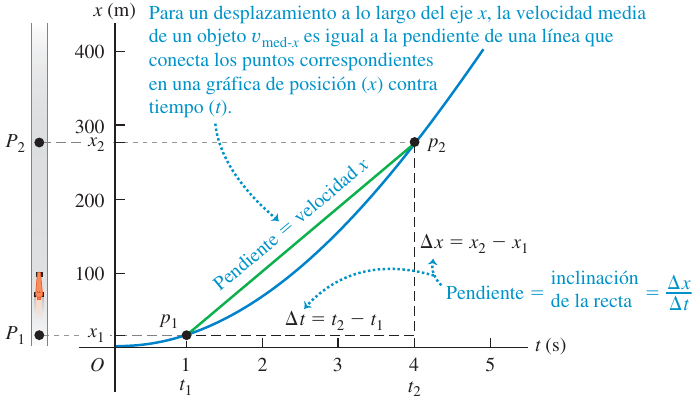
\includegraphics[width=0.85\textwidth]{figs/v_instantanea-1.png}
\end{center}
\cw{0.55}
{\small
\begin{itemize}
    \item La velocidad instantánea se obtiene como el límite al que se aproxima la velocidad media cuando el intervalo de tiempo es infinitamente pequeño:
    \[ \bm{v} = \lim_{\Delta t \rightarrow 0} \frac{\Delta \bm{r}}{\Delta t}i, \quad v_x = \lim_{t \rightarrow 0} \frac{\Delta x}{\Delta t} = \frac{dx}{dt} \mapsto \text{ ``derivada''} \]
    \item En la representación gráfica de $\bm{r}(t)$ la velocidad instantánea corresponde a la pendiente de la recta tangente a la curva en el punto de interés.
\end{itemize}
}
\end{columns}
\begin{center}
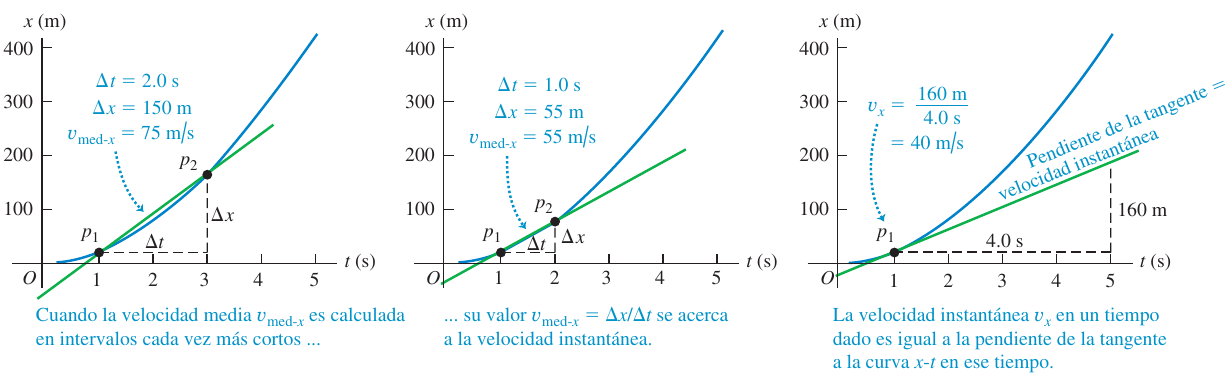
\includegraphics[width=0.9\textwidth]{figs/v_instantanea.png}
\end{center}
\end{frame}

\begin{frame}{Velocidad instantánea}
    \begin{center}
        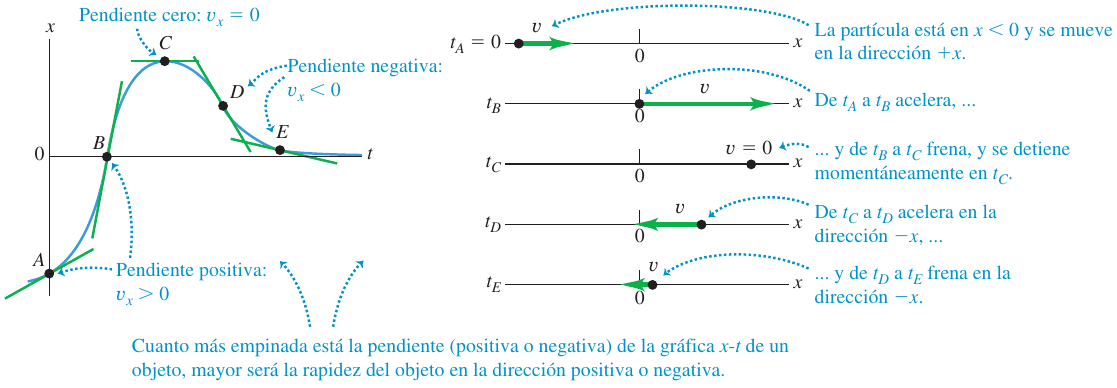
\includegraphics[width=1.0\textwidth]{figs/v_instantanea-2.png}
    \end{center}
\end{frame}

\begin{frame}{Ejemplo}
%{\small
    Un guepardo acecha \qty{20}{m} al este del escondite de un observador. En el tiempo $t = \qty{0}{s}$, el guepardo ataca a un antílope y empieza a correr en línea recta. Durante los primeros \qty{2}{s} del ataque, la coordenada $x$ del guepardo varía con el tiempo según la ecuación $x = \qty{20}{m} + (\qty{5}{m/s^2}) \, t^2$. a) Obtenga el desplazamiento del guepardo entre $t_1 = \qty{1.0}{s}$ y $t_2 = \qty{2.0}{s}$. b) Calcule la velocidad media en dicho intervalo. c) Calcule la velocidad instantánea en $t_1 = \qty{1.0}{s}$ tomando $\Delta t = \qty{0.1}{s}$, luego $\Delta t = \qty{0.01}{s}$, luego $\Delta t = \qty{0.001}{s}$. d) Deduzca una expresión general para la velocidad instantánea en función del tiempo y con ella calcule $v_x$ en $t = \qty{1.0}{s}$ y $t = \qty{2}{s}$. (Derivada de $t^n = n\, t^{n-1}$.)
%}
\begin{center}
    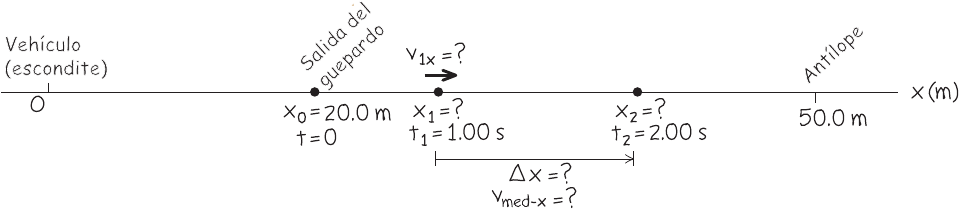
\includegraphics[width=0.9\textwidth]{figs/guepardo.png}
\end{center}
\end{frame}

\begin{frame}{Actividad}
    \begin{columns}
        \cw{0.4}
        \begin{center}
            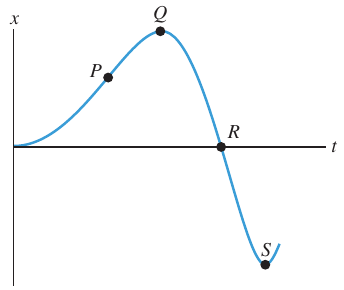
\includegraphics[width=0.7\textwidth]{figs/fig-04.png}
        \end{center}
        \cw{0.6}
        Ordene los valores de la velocidad $v_x$ de la partícula en los puntos $P$, $Q$, $R$ y $S$ del más positivo al más negativo. b) ¿En qué puntos $v_x$ es positiva? c) ¿En cuáles puntos $v_x$ es negativa? d) ¿En cuáles es cero? e) Ordene los valores de la \textbf{rapidez} de la partícula en los puntos $P$, $Q$, $R$ y $S$ del más rápido al más lento.
    \end{columns}
\end{frame}

\begin{frame}{Velocidad y aceleración}
\begin{columns} 
\cw{0.35}
\begin{center}
    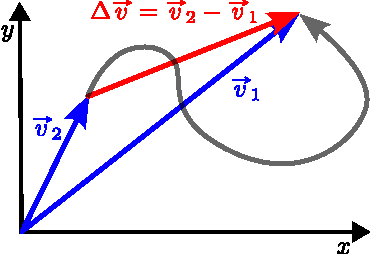
\includegraphics[width=0.9\textwidth]{figs/fig-05.pdf}
\end{center}
\cw{0.55}
\textbf{Aceleración media}
\begin{align*}
    \bm{a}_m &= \frac{\Delta \bm{v}}{\Delta t} \mapsto \text{ aceleración media} \\
    a_m &= \frac{\norm{\Delta \bm{v}}}{\Delta t} \mapsto \text{ norma o módulo}
\end{align*}
\end{columns}
\pause

\begin{example}
    Adela viaja en bici \qty{2.0}{h}. Inicia rumbo al este a \qty{10}{km/h}. Luego de muchas vueltas se encuentra viajando al norte a \qty{20}{km/h}. ¿Cuál fue su aceleración media?
    \begin{columns}
        \cw{0.35}
        \begin{align*}
            \bm{v}_1 &= (\num{10.0} \bm{i} + \num{0.0} \bm{j}) \unit{km/h} \\
            \bm{v}_2 &= (\num{0.0} \bm{i} + \num{20.0} \bm{j}) \unit{km/h} \\
            \bm{a}_m &= \frac{\bm{v}_2 - \bm{v}_1}{\Delta t} 
        \end{align*}
        \cw{0.65}
        \begin{align*}
             \bm{a}_m &= \frac{(-\num{10.0} \bm{i} + \num{20.0} \bm{j}) \unit{km/h}}{\qty{2.0}{h}} \\
                     &= (-\num{5.0} \bm{i} + \num{10.0} \bm{j}) \unit{km/h^2} \\
             a_m &= \norm{\bm{a}_m} = \sqrt{(\num{-5.0})^2 + \num{10.0}^2) \unit{km^2/h^4}} = \qty{11.18}{km/h^2}
        \end{align*}
    \end{columns}
\end{example}
\end{frame}

\begin{frame}{Velocidad y aceleración: caso unidimensional}
\begin{columns}
\cx
\begin{center}
    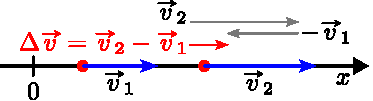
\includegraphics[width=1.0\textwidth]{figs/fig-06.pdf}
\end{center}
\begin{itemize}
    \item Aceleración media:
        \[ a_m = \frac{\Delta v}{|\delta t} = \frac{v_2 - v_1}{\Delta t} \] \\
        \item Módulo (norma): 
            \[ |a|  = \frac{|\Delta v|}{|\Delta t} = \frac{|v_2 - v_1|}{\Delta t} \]
    \end{itemize}
    \cx
    \begin{example}
        { \small Adela baja en bici por una pendiente recta hacia el este durante \qty{0.1}{h}. Inicia a \qty{10}{km/h}, acelera, aplica frenos varias veces y llega al final a \qty{50}{km/h}. ¿Cuál fue su aceleración media? Al día siguiente sube la pendiente sin pedalear. Antes toma mucha velocidad (\qty{60}{km/h}) y luego de \qty{0.2}{h} la bici se detiene por completo. ¿Cuál fue su aceleración media? }
        \begin{center}
            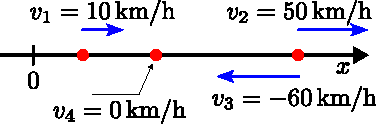
\includegraphics[width=0.7\textwidth]{figs/fig-07.pdf}
        \end{center}
        \begin{align*}
            a_{1 \rightarrow 2} = \frac{(\num{50} - \num{10})\unit{km/h}}{\qty{0.1}{h}} = \qty{400}{k/h^2} \\
            a_{3 \rightarrow 4} = \frac{(\num{-60} - \num{0}) \unit{km/h}}{\qty{0.2}{h}} = \qty{-300}{km/h^2}
        \end{align*}
    \end{example}
    \end{columns}
\end{frame}

\begin{frame}{Representación gráfica}
\begin{columns}
\cx
\begin{center}
    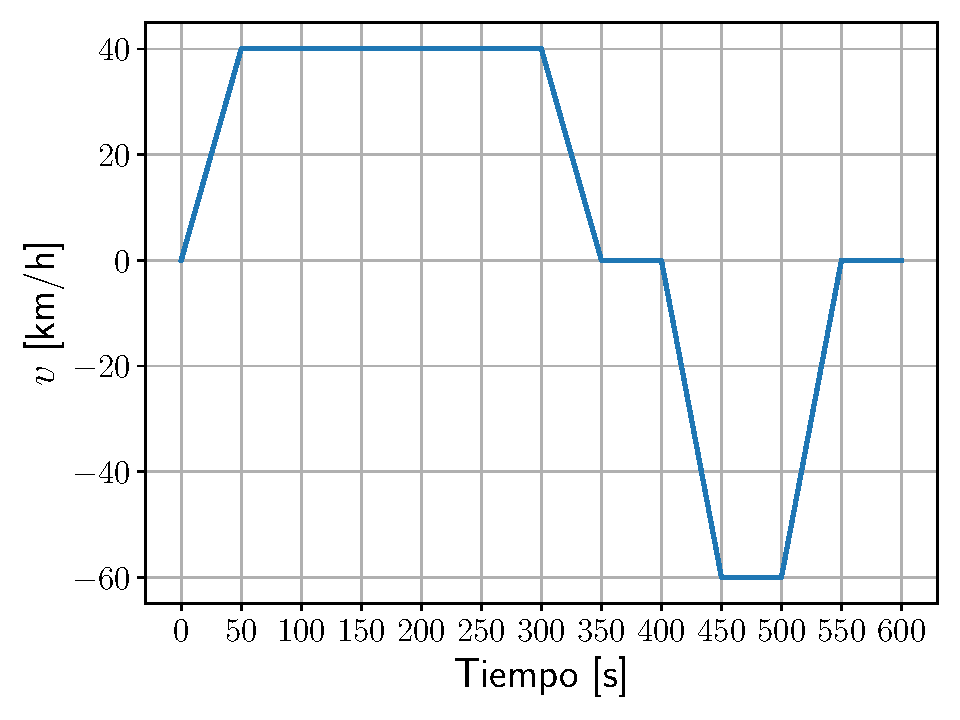
\includegraphics[width=0.9\textwidth]{figs/bruno-2.pdf}
\end{center}
\cx
Bruno sale en coche por una calle recta de oeste a este. El gráfico representa la velocidad de Bruno en cada momento.
{\small 
\begin{itemize}
    \item ¿Cuándo la rapidez fue de \qty{20}{km/h}? ¿Y cuando la velocidad fue de \qty{20}{km/h}?
    \item ¿Cuál era su velocidad \qty{200}{s} luego de partir? ¿Y a los \qty{325}{s}, y a los \qty{400}{s}?
 \item ¿En algún momento se detiene? ¿Cuándo? ¿Cuál es la máxima velocidad que alcanza? ¿Y la mínima? ¿Y la máxima rapidez?
\end{itemize}
}
\end{columns}
\begin{multicols}{2}
{ \small
\begin{itemize}
 \item ¿En qué dirección viaja a los $25$ s? ¿Y a los $325$ s? ¿Y a los $450$ s?
 \item ¿Cuánto dura el trayecto hacia el Este?
 \item ¿Al regreso hacia el oeste se detiene en el mismo lugar de donde partió el viaje?
 \item ¿Cuántos kilómetros recorrió en total?
 \item ¿Con qué aceleración media se mueve Bruno en cada tramo de su viaje?
 \item ¿Cuál es el módulo de la aceleración en cada tramo?
\end{itemize}
}
\end{multicols}
\end{frame}

\begin{frame}{Aceleración instantánea}
    \begin{center}
        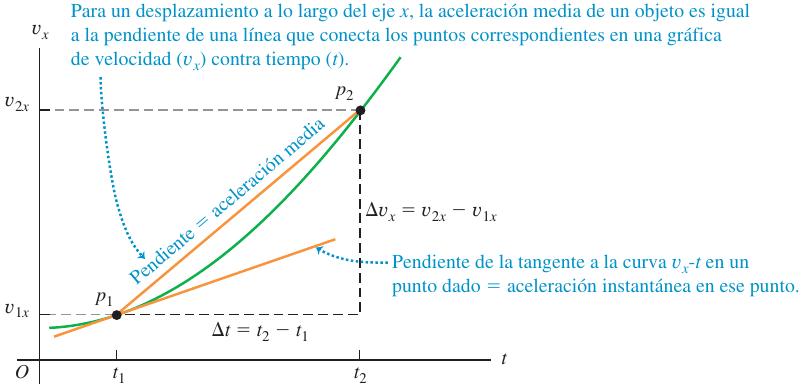
\includegraphics[width=0.7\textwidth]{figs/a_instantanea.png}
    \end{center}
    \[ \text{3D: } \bm{a} = \lim_{\Delta t \rightarrow 0} \frac{\Delta \bm{v}}{\Delta t}, \quad \text{1D: } a_x = \lim_{\Delta t \rightarrow 0} \frac{\Delta v_x}{\Delta t} = \frac{dv_x}{dt} \]
\end{frame}

\begin{frame}{Ejemplo:}
\small
\begin{columns}[t]
\cx
La velocidad $v_x$ de un móvil en función del tiempo esta dada por
\[ v_x = \qty{60}{m/s} + (\qty{0.50}{m/s^3}) t^2\]
a) Calcule el cambio de velocidad del móvil entre el intervalo $t_1 + \qty{1.0}{s}$ y $t_2 = \qty{3.0}{s}$. b) Calcule la aceleración media en ese intervalo. c) Obtenga la aceleración instantánea en $t_1$ tomando $\Delta t$ primero como \qty{0.1}{s}, después como \qty{0.01}{s} y luego como \qty{0.001}{s}. d) Deduzca una expresión para la aceleración instantánea en cualquier instante y úsela para obtener la aceleración en $t_1$ y $t_2$.
\pause

\vspace{1em}
a)
\begin{align*}
    v_{1x} &= \qty{60}{m/s} + (\qty{0.50}{m/s^3})(\qty{1.0}{s})^2 = \qty{60.5}{m/s} \\
    v_{2x} &= \qty{60}{m/s} + (\qty{0.50}{m/s^3})(\qty{3.0}{s})^2 = \qty{64.5}{m/s} \\
    \Delta v_x &= v_{2x} - v_{1x} = \qty{4.0}{m/s}
\end{align*}

\cx
b)
\[ a_{mx} = \frac{v_{2x} - v_{1x}}{t_2 - t_1} = \frac{\qty{4.0}{m/s}}{\qty{2.0}{s}} = \qty{2.0}{m/s^2} \]

\vspace{1em}
c)
\begin{center}
    \begin{tabular}{lccc}
        \toprule
        $\Delta t$ (\unit{s}) & $0.1$ & $0.01$ & $0.001$ \\
        $a_{mx}$ (\unit{m/s^2}) & $1.05$ & $1.005$ & $1.0005$ \\
        \bottomrule
    \end{tabular}

\vspace{1em}
d) $a_x = dv_x/dt$, la derivada de una constante es cero y la de $t^2$ es $2 t$:

\begin{align*}
    a_x &= \frac{dv_x}{dt} = \frac{d}{dt}[\qty{60}{m/s} + (\qty{0.50}{m/s^3}) t^2] \\
        &= (\qty{0.50}{m/s^3})(2 t) = (\qty{1.0}{m/s^3}) t \\
    t=\qty{1.0}{s}: a_x &= (\qty{1.0}{m/s^3})(\qty{1.0}{s}) = \qty{1.0}{m/s^2} \\
    t=\qty{3.0}{s}: a_x &= (\qty{1.0}{m/s^3})(\qty{3.0}{s}) = \qty{3.0}{m/s^2} \\
\end{align*}
\end{center}
\end{columns}
\end{frame}

\begin{frame}{Posición, velocidad y aceleración 1D}
    \begin{center}
        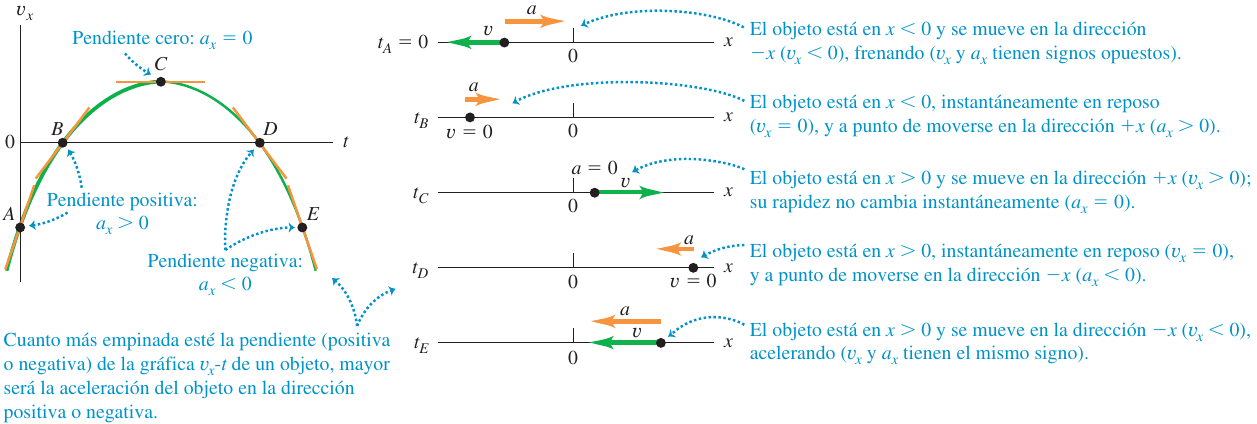
\includegraphics[width=1.0\textwidth]{figs/xva.png}
    \end{center}
\end{frame}

\begin{frame}{Posición, velocidad y aceleración 1D}
    \begin{center}
        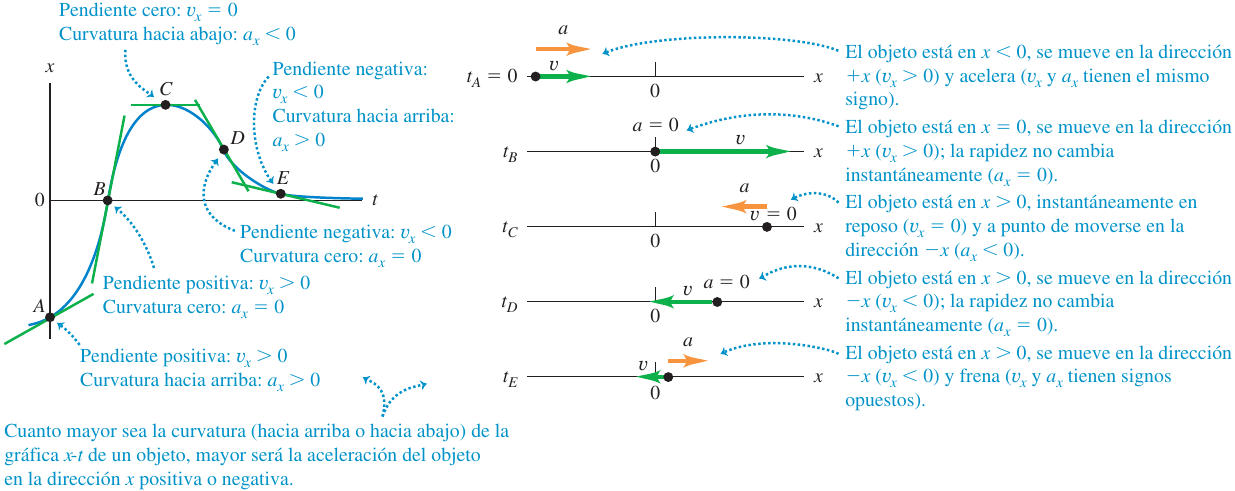
\includegraphics[width=1.0\textwidth]{figs/xva-2.png}
    \end{center}
\end{frame}

\begin{frame}{Movimiento rectilíneo con aceleración constante}
\begin{columns}
\cx
\begin{center}
    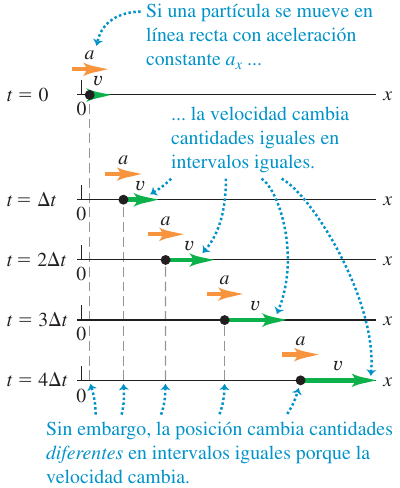
\includegraphics[width=0.7\textwidth]{figs/mrua-1.png}
\end{center}
\cx
\begin{center}
    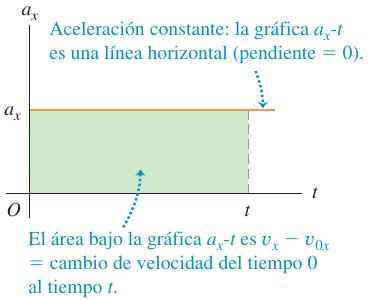
\includegraphics[width=0.6\textwidth]{figs/mrua-2.png}
\end{center}

Con \textbf{aceleración constante:}
\begin{equation} 
    a_x = \frac{v_x - v_{0x}}{t - 0} \Rightarrow \boxed{v_x(t) = v_{0x} + a_x \, t} 
\label{eq:vt}
\end{equation}
\end{columns}
\end{frame}

\begin{frame}{Movimiento rectilíneo con aceleración constante}
\begin{columns}
 \cw{0.3}
\begin{center}
    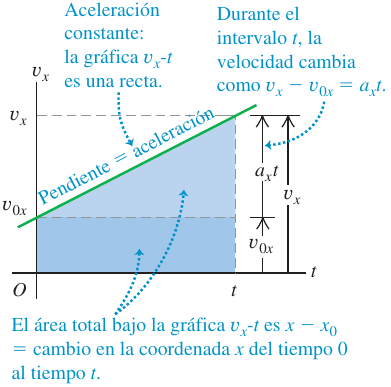
\includegraphics[width=0.9\textwidth]{figs/mrua-3.png}
\end{center}
 \cw{0.7}
Con \textbf{aceleración constante:}
\begin{align*} 
v_{mx} &= \frac{x - x_0}{t}, \text{y también}\\
v_{mx} &= \frac{v_{0x} + v_x}{2} = \frac{1}{2} (v_{0x} + v_{0x} + a_x \, t) = v_{0x} + \frac{1}{2} a_x \, t
\end{align*}
Igualando y despejando $x$:
\begin{equation} 
\boxed{ x = x_0(t) + v_{0x} \, t + \frac{1}{2} a_x \, t^2 } 
\label{eq:xt}
\end{equation}
\end{columns}
\end{frame}

\begin{frame}{Interpretación gráfica}
\begin{center}
    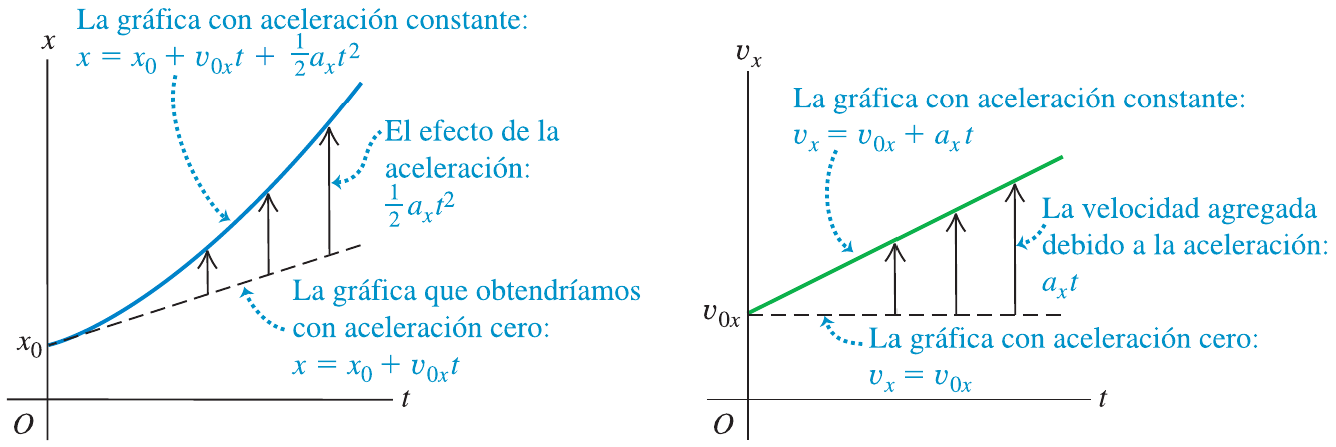
\includegraphics[width=0.9\textwidth]{figs/mrua-4.png}
\end{center}
\pause

{\small
Despejando $t$ de \eqref{eq:vt}, reemplazando en \eqref{eq:xt} y simplificando:
\begin{columns}[t]
    \cw{0.45}
\begin{align*}
    t &= \frac{v_x - v_{0x}}{a_x} \\
    x &= x_0 + v_{0x} \left(\frac{v_x - v_{0x}}{a_x}\right) + \tfrac{1}{2} a_x \left(\frac{v_x - v_{0x}}{a_x}\right)^2
\end{align*}
    \cw{0.5}
Pasando $x_0$ al primer miembro y multiplicando por $2 a_x$:
\begin{align}
    2 a_x(x - x_0) &= 2 v_{0x} v_x - 2 v_{0x}^2 + v_x^2 -2 v_{0x} v_x + v_{0x}^2 \notag \\
    v_x^2 &= v_{0x}^2 + 2 a_x (x - x_0) \\
x-x_0 &= \left(\frac{v_{0x} + v_x}{2} \right) t
\end{align}
\end{columns}
}
\end{frame}

\end{document}

